The functions associated with the poly-mod section are very powerful and these functions set the synth apart from many other synths. In essence, poly-mod provides tools for non-linear modulation, e.g. to cross-modulate the two oscillators per voice and also to modulate the filter cut-off frequency by VCO B. 

Modulating the oscillator frequency and cut-off frequency using a \textit{low frequency oscillator (LFO)} is a common feature. An LFO does not operate in the audible frequency range and it is also fixed in frequency, e.g. independent from the note played. Poly-mod is different in that the modulation itself is in the audible range and the non-linearity changes the frequency spectrum drastically. In one or the other form the resulting effect may be compared to FM synthesis, althought in the Prophet 600 it is more raw and fully analog. Importantly, similar to the sync function the oscillator cross-modulation is implemented in the hardware.

The poly-mod control can be found in the poly-mod section of the panel. There are two modulation sources. The \textbf{OSC B} dial sets how strongly the sonic output of VCO B influences poly-mod targets. 

\scalebox{0.4}{
  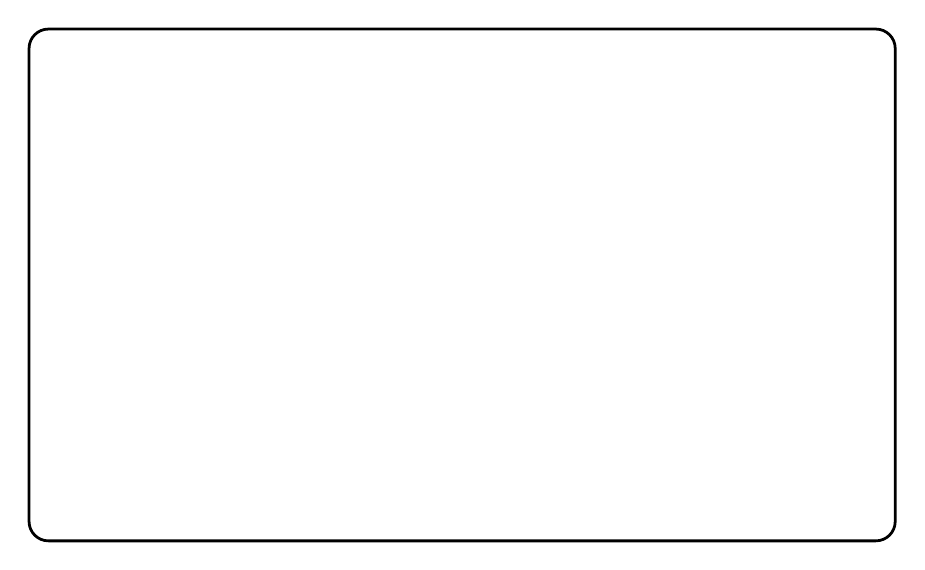
\begin{tikzpicture}[scale=0.8]
    \node[rectangle, draw, rounded corners=7pt, line width=1pt, minimum width = 11cm, minimum height = 6.5cm, anchor = south west] (r) at (0,0) {};
    \prophetpotbiplar{4cm,4cm}{ENVELOPE}{75}
    \prophetpot{10cm,4cm}{OSC B}{75}
  \end{tikzpicture}
}

Before looking at the second source (envelope) it is instructive to consider the effect of VCO B modulation on the two targets, which can be selected using the dedicated switches:

\begin{itemize}
  \item When setting the \textbf{Frequency A} switch to \textit{on}, VCO B modulates the frequency of VCO A. In different variants this is also known as frequency modulation, or short: FM. Depending on the modulation strength the result is a wide and rich freuency spectrum which contains among others the sum and difference of multiples of the two oscillators frequencies . The spetrum strongly depends on the frequency difference and may be totally non-harmonic but also harmonic for carefully adjusted frequency settings. Typical spectra are often described as bell sounding. Note that in contrast to FM synthesizers which use highly accurate sin waves, the oscillator output of the Prophet does not provide the same basic accuracy and the available waveforms already contain many higher harmonics. Therefore the FM result in the Prophet 600 is typically more drastic and dirtier and requires classic subtractive methods for shaping the sound, e.g. the application of the low pass filter. 
  \item When setting the \textbf{Filter} switch to \textit{on}, VCO B modulates the cut-off frequency of the VCF. Like frequency modulation this is a non-linear modulation but with a less drastic effect than oscillator frequency modulation. It can produce a wide frequency spectrum which may or may not be harmonic, depending on the relative frequenc of VCO A and VCO B. The effect is more pronunced at low filter cutt-off frequencies. The resonsance also has a strong effect.  
\end{itemize}

The second modulation source in the poly-mod envelope as set by the \textbf{Envelope} dial. This activates a pitch modulation of VCO A using an envelope is the Frequency switch is \textit{on} \footnote{Note that the poly-mod envelope can only affect the freqnecy of VCO A. The cut-off frequency is already modulated by the filter envelope so the poly-mod envelope will have no effect on the filter cut-off frequency even if this target is activated.}. The dial provides negative (inverse modulation) and positive values. The pitch modulation by envelope is not a cross-modulation. However, the association of pitch modulation with poly-mod is still appropriate because with cross-modulation the frequency has a drastic effect on the sound, ranging from apocalyptic noice through bell sounds to delicate transients (attack phase of a sound). Of course, with poly-mod activated, LFO and vibrato also begin to have an inflence on the frequency spectrum, which can be drastic. However, envelope modulation provides a means for sculping sounds. In particular, the way humans perceive natural sounds is often related to frequency characteristics in the transients (typically short lived high frequency components) in the attack and decay phases of the sound. This is best modelled using an envelope. Whether the filter envelope or the assignable envelope is routed to this modulation is controlled by the additional patch parameter \textbf{(555) Envelope Routing}. Prior to version 2.2 it was the filter envelope which was "hard wired" to poly-mod. Having the option to use a different envelope, open new patch possibilities. The Envelope Routing options are as follows. 

\begin{itemize}
  \setlength\itemsep{0cm}
  \item \textit{standard}: In this "standard" routing the amplitude is modulated by the assignable envelope and the poly-mod is modulated by the filter envelope. This is the setup of the original Prophet 600. 
  \item \textit{poly-amplitude}: In this routing both the amplitude and the poly-mod are modulated by the assignable envelope. 
  \item \textit{poly}: In this routing the amplitude is modulated by the filter envelope and the poly-mod is modulated exclusively by the assignable envelope. Therefore the poly-mod modulation is completely free at the expense of having filter and amplitude tied together.
  \item \textit{gate}: In this routing the amplitude is not modulated at all, but behaves like a gate (similar to electronic organs). The poly-mod is modulated exclusively by the assignable envelope. Therefore the poly-mod modulation is completely free at the expense of have a less dynamic sound evolution.
\end{itemize}  

Note that sync'ing VCO A to VCO B (Sync switch on the panel section of oscillator A) is also an important variant of cross-modulation. The sync function can be combined with frequency modulation. In combination with pitch modulation of VCO A sync can produce intereseting transients.  

Note that poly-mod is very tuning sensitive and that it maybe necessary to retune the synth more often when using extreme poly-mod settings.

Using poly-mod in combination with oscillator sync, different modulations strengths for different oscillator pitches with different filter and modulation shapes is a ver wide field of experimentation. Here are some ideas as potential starting points

\begin{itemize}
  \item Set the envelope routing to \textit{standard}, tune both oscillators to the same frequency, in the poly-mod scetion turn source VCO B to zero and deactivate the filter modulation. Then set VCO A to sync and experiment with the poly-mod envelope source amount. This produces a sync whic, for high envelope amounts, can be tuned to a quite harsh synth solo sound.
  \item ... (describe a few generic settings, e.g. also bells, UFO etc.)
\end{itemize} 
